% !TEX root = ../main.tex
\section{Experimental Setup}
\label{sec:setup}

\subsection{Dataset and Settings}
\label{sec:setup-dataset}
We use the dataset introduced in Heo et al.~\cite{heo2025study} for our experiments. The dataset has a total of 6,600 issue reports gathered from eleven active open-source projects:
\texttt{ansible/ansible}, \texttt{bitcoin/bitcoin},
\texttt{dart-lang/sdk}, \texttt{dotnet/roslyn},
\texttt{facebook/react}, \texttt{flutter/flutter},
\texttt{kubernetes/kubernetes}, \texttt{microsoft/TypeScript},
\texttt{microsoft/vscode}, \texttt{opencv/opencv}, and
\texttt{tensorflow/tensorflow}. Each project has 600 issue reports
with an equal distribution across the labels
(\textit{bug, feature, question}). To support their LLM fine-tuning
method, Heo et al. divided the dataset into 50/50 train and test
splits, stratified by project and label. This results in 300 train
and 300 test issue reports per project.

We also adopt Heo et al.'s project-specific (PS) and project-agnostic
(PA) configurations to examine how data scope affects IRC performance.
In the PS setting, each project's train and test data are used in
isolation, resulting in eleven different train-test pairs. In the PA
setting, the train splits of all projects are merged into a single
training set of 3,300 issue reports. In both configurations, \ragtag
and \votag only use the training splits as their retrieval index to
ensure fair comparison with the fine-tuning baseline. \Cref{fig:ps-pa} illustrates the difference between the two settings.

\begin{figure}[t]
    \centering
    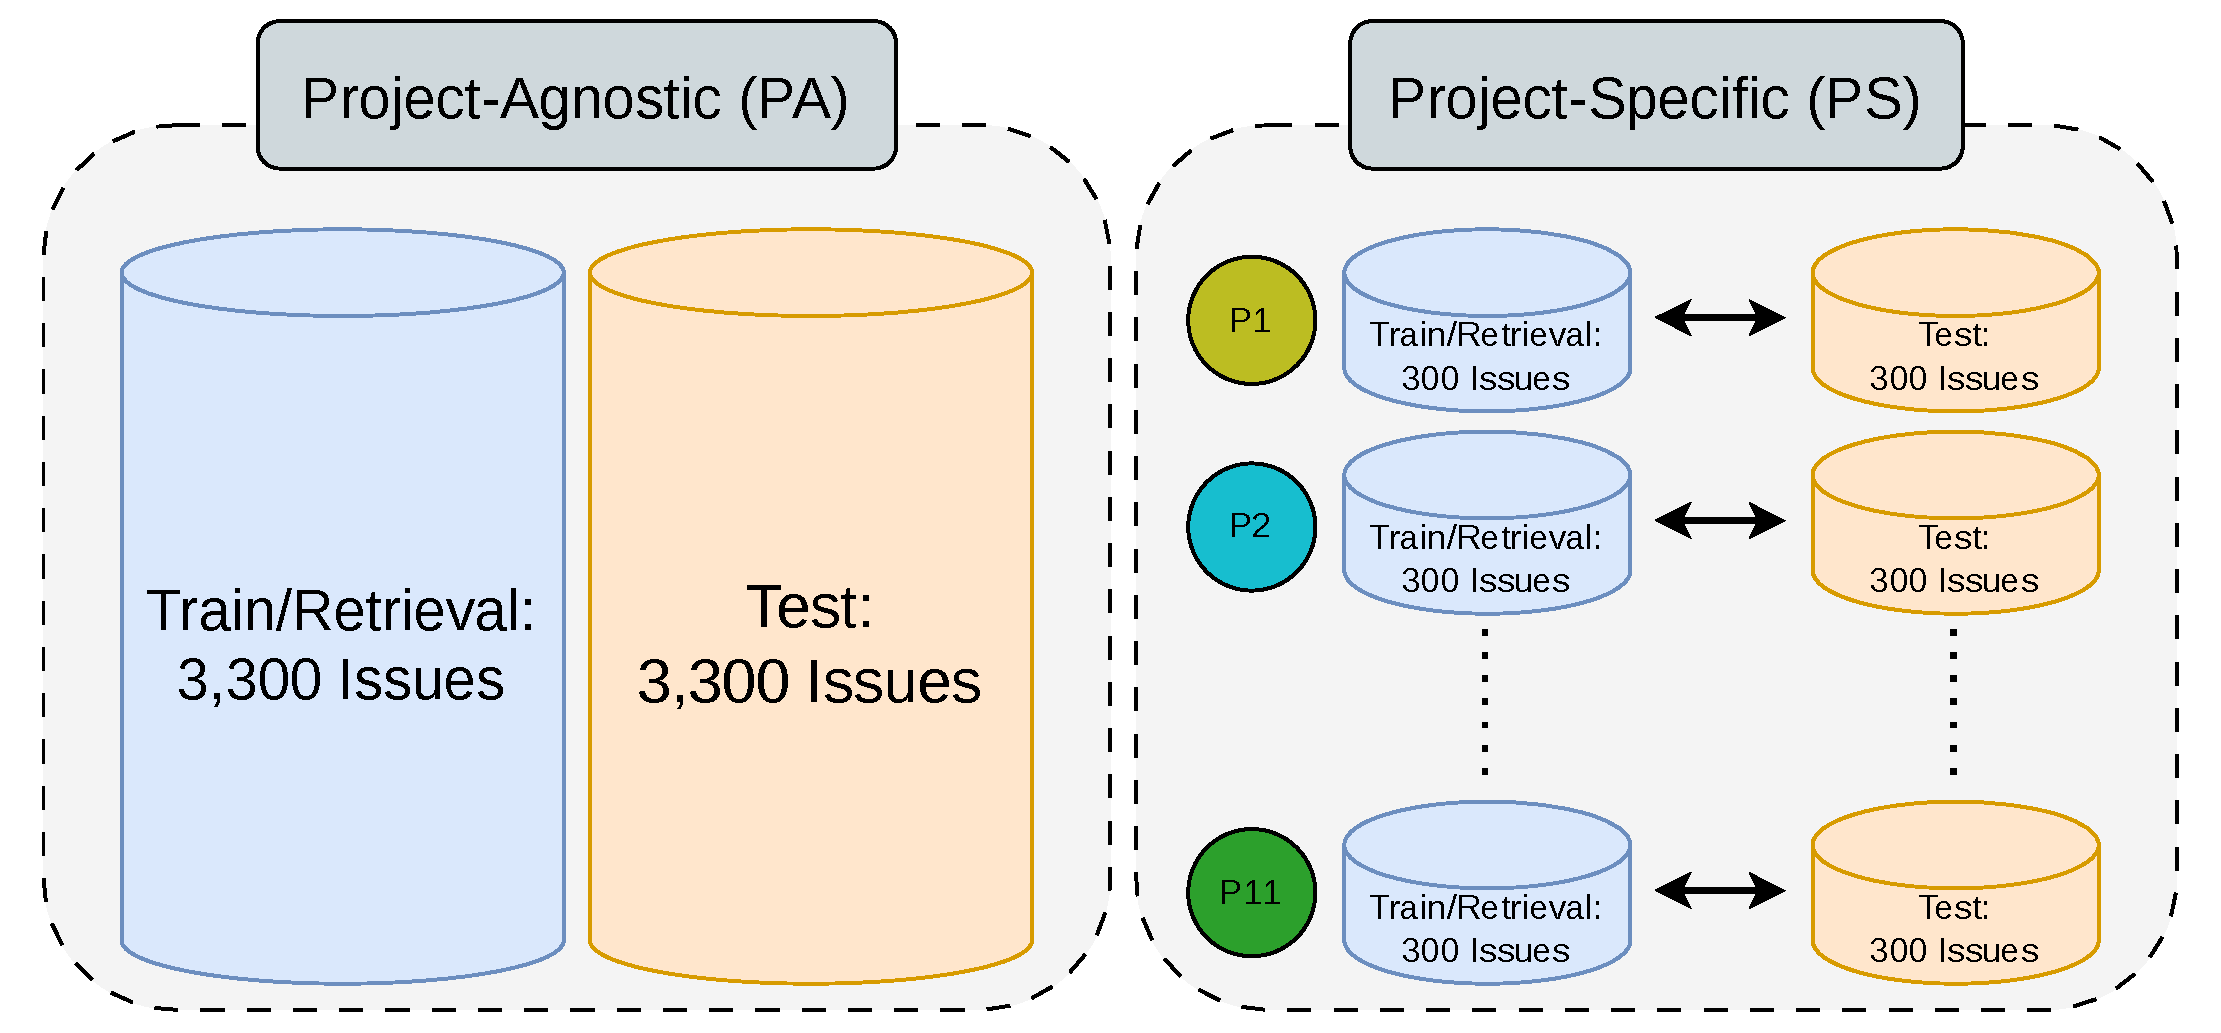
\includegraphics[width=0.8\linewidth]{figures/PS-PA.pdf}
    \caption{Project-Specific (PS) vs.\ Project-Agnostic (PA) data scope settings.}
    \label{fig:ps-pa}
\end{figure}

\subsection{Models}
\label{sec:setup-models}
We use the Qwen2.5-Instruct model family~\cite{yang2024qwen25} in our evaluations with four different parameter sizes: 3B, 7B, 14B, and 32B. Qwen2.5 is an open-source LLM with strong performance on general-purpose benchmarks. Using the same model at different parameter sizes isolates the effect of model scale from model architecture across LLM-based IRC approaches.


\subsection{Evaluation Metrics}
\label{sec:setup-metrics}
We report the per-class $F_1$ and the macro-averaged $F_1$ over the three classes (\texttt{bug}, \texttt{feature}, \texttt{question}). The macro $F_1$ is calculated over the total 3{,}300-issue test set in all settings. We also report the rate of outputs that fail to parse to a valid label (\textit{invalid rate}). For statistical significance checks, we report paired bootstrap 95\% confidence intervals on the macro $F_1$ differences between methods.

\subsection{Hardware Setup}
\label{sec:setup-hardware}
The experiments were conducted on a machine with one NVIDIA L40 GPU (48~GB VRAM), 8~allocated CPU cores from an Intel Xeon Scalable processor, and 64~GiB of system RAM.
